% Number 320
% CVPMG Units
% Chase after distance pause: problem-solving
% JG

% Watermark
\AddToShipoutPicture*{\BackgroundPic}

\addtocounter {ProbNum} {1}

%\begin{floatingfigure}[r]{.3\textwidth}
%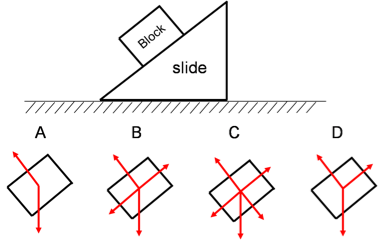
\includegraphics[scale=.4]{/Users/jgates/desktop/latex/pics/incline3.png}
%\end{floatingfigure}
 
{\bf \Large{\arabic{ProbNum}}}A real police car chases down a stolen sturgeon truck.  The police car is sitting by the side of the road when the truck flies by at ${35~\tfrac{m}{s}}$.  Assume that the police officer reacts after the truck is 150 meters past her and gets up to speed instantly.  
 
%\begin{center}
%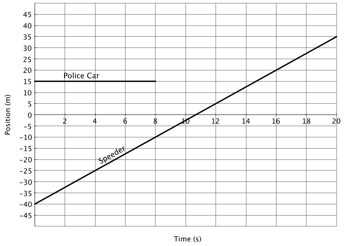
\includegraphics[scale=.87]{/Users/jgates/desktop/latex/pics/cvpm2.png}
%\end{center}

\bigskip
How fast does she need to go in order to catch the truck within 2 minutes? Use graphical problem-solving.
 
\vfill

\newpage